\documentclass[journal]{IEEEtran}

\usepackage[T1]{fontenc}

\usepackage{cite}
\usepackage{amsmath}
\interdisplaylinepenalty=2500
\usepackage{amssymb}
\usepackage{amsthm}
\usepackage{graphicx}
\usepackage{booktabs}
\usepackage{array}
\usepackage[caption=false,font=footnotesize,labelformat=simple,justification=centering]{subfig}
\usepackage{url}
\usepackage[hidelinks]{hyperref}
% URLs break only after a slash or a dot, never right after "https:" (":" is a relation by default, and the
% url package prefers a break there); as an "open" character it allows no break.
\def\UrlBigBreaks{}
\def\UrlBreaks{\do\/\do\.\do\-\do\_}
\def\UrlNoBreaks{\do\(\do\[\do\{\do\<\do\:}

% Shared notation for every section (do not redefine elsewhere)
\newcommand{\BIG}{\mathsf{B}}                       % value of a passed pawn, B = 256
\newcommand{\pos}[1]{\texttt{#1}}                   % pawn list, e.g. \pos{W a2 c2 / B b7 d7}
\newcommand{\fen}[1]{\texttt{\small #1}}
\newcommand{\lab}[1]{\textsf{\footnotesize$\langle$#1$\rangle$}}   % evidence label: \lab{P}, \lab{S}, \lab{C2}, \lab{C1}, \lab{Conj}
\newcommand{\nim}[1]{\mathord{\star#1}}             % nimbers, as in the 2025 paper: \star, \nim{2}
\newcommand{\upsec}{\mathord{\uparrow^{2}}}         % up-second {0 | down star}
\newcommand{\tinyg}[1]{\operatorname{tiny}(#1)}
\newcommand{\game}[2]{\{\,#1 \mid #2\,\}}
\newcommand{\ggame}[2]{\{\,#1 \parallel #2\,\}}
\newcommand{\cyl}[1]{C_{#1}}                        % n-file cylinder
\newcommand{\flatb}[1]{F_{#1}}                      % n-file flat board
\newcommand{\repourl}{https://github.com/aritroBh/cylindrical-chess-cgt}


% Placeholder for the anonymous repository link (anonymous build). Replace the text by
% \url{https://anonymous.4open.science/r/<id>} once the mirror exists.
\newcommand{\anoncodeurl}{anonymized repository link}

% Two builds. tog.tex is the named build. tog_review.tex defines \anonbuild and inputs this file,
% which gives the double-anonymous review build for IEEE Transactions on Games.
% \submittedtrue adds IEEE's preprint notice to the named build. Turn it on only once the paper has been
% submitted to the IEEE (GUIDELINES F); it never appears in the review build.
\newif\ifsubmitted
\submittedfalse
\ifdefined\anonbuild
  \newcommand{\codeurl}{}
  \newcommand{\codeavail}{available at \anoncodeurl}
  \newcommand{\bytheauthor}{}
  \newcommand{\studyauthor}{Anonymous}
  \newcommand{\studytitle}{Title withheld for review}
  \hypersetup{pdftitle={Combinatorial Game Values and Tablebases for Chess Endgames on a Cylindrical Board}, pdfauthor={}}
\else
  \newcommand{\codeurl}{\url{https://github.com/aritroBh/cylindrical-chess-cgt}}
  \newcommand{\codeavail}{available at \codeurl}
  \newcommand{\bytheauthor}{ by the author}
  \newcommand{\studyauthor}{A.~Bhattacharjee}
  \newcommand{\studytitle}{Analysis of chess endgames on a cylindrical chessboard}
  \hypersetup{pdftitle={Combinatorial Game Values and Tablebases for Chess Endgames on a Cylindrical Board}, pdfauthor={Aritro Bhattacharjee}}
\fi

% The sections use the subcaption-style environment
%   \begin{subfigure}[pos]{width} ... \caption{...}\label{...} \end{subfigure}.
% IEEEtran's captions are kept by implementing it with subfig's \subfloat (caption=false), as the
% IEEEtran HOWTO recommends. A subfigure is labelled (a) and referenced as Fig. 3(a).
\renewcommand{\thesubfigure}{(\alph{subfigure})}
\makeatletter
\newsavebox{\sf@box}
\newcommand{\sf@setcap}[2][]{\gdef\sf@cap{#2}}
\newcommand{\sf@setlab}[1]{\gdef\sf@lab{#1}}
\newenvironment{subfigure}[2][c]{%
  \gdef\sf@cap{}\gdef\sf@lab{}%
  \begin{lrbox}{\sf@box}\begin{minipage}[#1]{#2}%
  \let\caption\sf@setcap\let\label\sf@setlab}%
  {\end{minipage}\end{lrbox}%
   \ifx\sf@lab\@empty\def\sf@labcmd{}\else\edef\sf@labcmd{\noexpand\label{\sf@lab}}\fi
   \ifx\sf@cap\@empty\subfloat[]{\usebox{\sf@box}\sf@labcmd}%
   \else\subfloat[\sf@cap\sf@labcmd]{\usebox{\sf@box}}\fi}
\makeatother

% One counter for all numbered statements, through the whole paper, in IEEE style:
% an indented italic head ending in a colon ("Theorem 2 (Cut lemma; [P]):"). A head whose note is
% only an evidence label prints it without parentheses ("Proposition 4 [P]:").
\makeatletter
\def\ieeethmnote#1{\ieee@thmnote#1\@empty\@nil}
\def\ieee@thmnote#1#2\@nil{\ifx#1\lab\expandafter\@firstoftwo\else\expandafter\@secondoftwo\fi
  {\lab#2}{(#1#2)}}
\makeatother
\newtheoremstyle{ieeeplain}{3pt}{3pt}{\itshape}{\parindent}{\itshape}{:}{0.5em}%
  {\thmname{#1}\thmnumber{ #2}\thmnote{ \ieeethmnote{#3}}}
\newtheoremstyle{ieeedef}{3pt}{3pt}{\normalfont}{\parindent}{\itshape}{:}{0.5em}%
  {\thmname{#1}\thmnumber{ #2}\thmnote{ \ieeethmnote{#3}}}
\theoremstyle{ieeeplain}
\newtheorem{theorem}{Theorem}
\newtheorem{lemma}[theorem]{Lemma}
\newtheorem{proposition}[theorem]{Proposition}
\newtheorem{corollary}[theorem]{Corollary}
\newtheorem{conjecture}[theorem]{Conjecture}
\theoremstyle{ieeedef}
\newtheorem{definition}[theorem]{Definition}
\newtheorem{remark}[theorem]{Remark}
% Proofs use IEEEtran's proof layout; \begin{proof}[Proof sketch] prints "Proof sketch:".
\renewenvironment{proof}[1][Proof]{\begin{IEEEproof}[#1]}{\end{IEEEproof}}

\hyphenation{tr\'e-bu-chet tr\'e-bu-chets table-base table-bases}

\begin{document}

\title{Combinatorial Game Values and Tablebases for Chess Endgames on a Cylindrical Board}

\ifdefined\anonbuild
\author{Anonymized for review}
\markboth{IEEE Transactions on Games}{Chess Endgames on a Cylindrical Board}
\else
\ifsubmitted
  \newcommand{\ieeenotice}{\thanks{This work has been submitted to the IEEE for possible publication.
    Copyright may be transferred without notice, after which this version may no longer be accessible.}}
\else
  \newcommand{\ieeenotice}{}
\fi
\author{Aritro~Bhattacharjee%
\ieeenotice
\thanks{The author is with the University of Illinois Urbana-Champaign, Urbana, IL 61801 USA (e-mail: aritro.sonu@gmail.com).}}
\markboth{IEEE Transactions on Games}%
{Bhattacharjee: Chess Endgames on a Cylindrical Board}
\fi

\maketitle

\begin{abstract}
Cylinder chess joins the a-file to the h-file, leaving no side edges or corners. We study king-and-pawn
endgames with combinatorial game theory after Elkies: a passed pawn wins, and the kings are frozen in a mutual
zugzwang worth zero. We make the passed-pawn test respect en passant, and give conditions for frozen kings
to match chess. Under this test and the count rule, no position of at most six pawns on an ordinary board of any width has a
nimber above star; with seven, star two appears once, plus its color-reversed
twin, confirmed by three programs; its real-chess value is open. In pawn-only whole-board rings, star two needs six pawns on
three files and, from ten files on, one per file (proof sketched); on seven files ten-pawn rings reach star
three. We find positions with a legal pawn history worth one-eighth, up-second star and Tiny 1; with frozen kings
and queen promotions only, the one-eighth position's tablebase-backed oracle value is one-eighth. On the cylinder king and
rook rarely force mate, but opposite-colored bishops can. We correct earlier work on cylinder Dawson's chess: the
ring is a first-player win exactly when the strip three files shorter has Grundy value zero.
\end{abstract}

\begin{IEEEkeywords}
Chess, combinatorial game theory, endgame tablebases, game solving, nimbers.
\end{IEEEkeywords}


\section{Introduction}\label{sec:intro}

\IEEEPARstart{C}{ylinder} chess is ordinary chess on a board whose a-file and h-file are joined
\cite{Pritchard}: a white pawn on h4 can capture on a5, a king on a1 can step to h2, and there are no side edges or
corners (Fig.~\ref{fig:ring}). We use combinatorial game theory (CGT) to study its king-and-pawn endgames.

\begin{figure*}[!t]
\centering
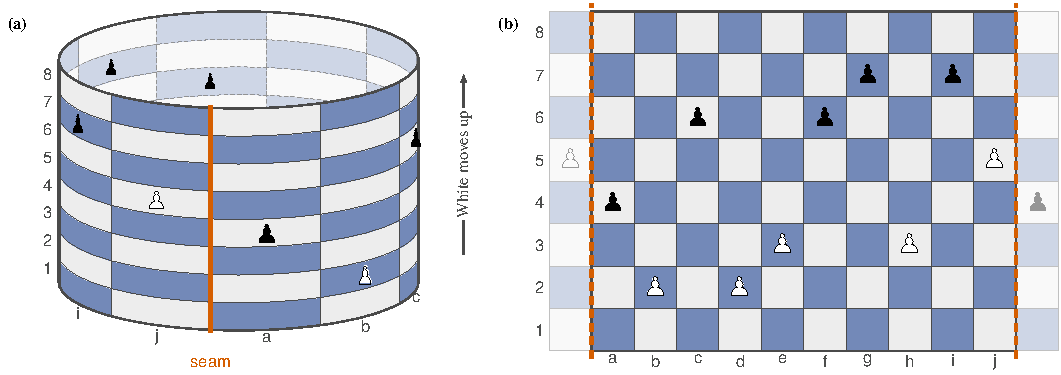
\includegraphics{figures/f1_ring_cylinder_wide.pdf}
\caption{Ring $M_{10}$ on the cylinder $\cyl{10}$. (a)~Perspective view; the seam between files j and a (orange)
faces the viewer, and the far wall is dashed and faded. Only the pawns that can be seen are drawn: 7 of the 10.
(b)~The same position unrolled, with all ten pawns, one per file; file j is next to file a across the dashed
seam, and the faded columns repeat j and a. White moves up. The position has value $\nim{2}$
(Section~\ref{sec:star2-rings}).}
\label{fig:ring}
\end{figure*}

Under normal play the player who cannot move loses; CGT gives each position a value, and a sum of independent
games has the sum of their values \cite{ONAG,WinningWays,Siegel2013}. Chess can be drawn and its kings roam,
yet Elkies \cite{Elkies1996} showed that many pawn endgames split into local fights with exact values, under
two conventions: a passed pawn wins, and is worth a large number $\pm\BIG$; and the kings stand in a mutual
zugzwang, the \emph{tr\'ebuchet}, worth $0$.

The cylinder changes this picture in three ways. There are no rook pawns, and shifting a position sideways
does not change its value. A position with a pawn on every file, a \emph{ring}, has no edge at which to cut
it, and no room for frozen kings, so ring values are values of the pawn-only model. And the corners that decide
mates and fortresses are gone.

Elkies built higher nimbers on large boards from Dawson's pawn game \cite{Elkies2002,Dawson1935}, and
Drummond-Cole built positions of value $\nim{2}$ in chess with the help of pieces other than kings and
pawns~\cite{DrummondCole2005}. We ask whether $\nim{2}$ (Section~\ref{sec:notation}) occurs in a king-and-pawn
endgame on an 8-rank board, the \emph{$\nim{2}$ question}, and whether real chess agrees.

This paper extends an unpublished 2025 study of the basic values\bytheauthor~\cite{Study2025}: we check
every position by computer, correct its errors (Sections~\ref{sec:sums} and~\ref{sec:dawson}) and carry
the analysis on, in the position-by-position format of Wu, Y\"u and Landry~\cite{WuYuLandry2010}. Results carry
labels: \lab{P}, proved here; \lab{S}, proof sketched here, with a full AI-written, AI-refereed proof in the supplement;
\lab{C2}, two separately written programs agree, the second from the rules alone (ours are AI-written; Section~S17); \lab{C1}, one
program; \lab{Conj}, a conjecture. Our contributions are:
\begin{itemize}
\item \emph{Model and kings} (Sections~\ref{sec:rules}, \ref{sec:kings} and~\ref{sec:sums}): a passed-pawn
  test that respects en passant, a cut lemma \lab{P}; conditions (V1)--(V3) under which a frozen tr\'ebuchet gives
  the result of the whole-board pawn game \lab{S}, and (V4) for the $\pm\BIG$ value \lab{S}; a sum-safety
  theorem \lab{S}; and a position showing that checking only the top-level components is not enough \lab{C2}.
\item \emph{Small values} (Sections~\ref{sec:basic}, \ref{sec:atlas} and~\ref{sec:targets}): cylinder-only values come from rings
  \lab{P}; $1/8$ and $\upsec\star$ \lab{C2}, and Tiny~1 \lab{C1}, occur in 10-man positions with a legal pawn
  history.
\item \emph{The $\nim{2}$ question} (Section~\ref{sec:star2}): in the default setting (count rule, e.p.-aware test; Section~\ref{sec:ep}) no $\nim{2}$ has six
  pawns or fewer on ordinary boards of any width, but $\nim{2}$ appears with seven \lab{C2}; in the pawn-only
  model a six-pawn ring suffices on $\cyl{3}$ \lab{C2}, a ring needs ten on $\cyl{7}$ to $\cyl{10}$ \lab{C2}
  and only $n$, one per file, on every $\cyl{n}$ with $n\ge10$ as a whole-board game \lab{S}; on $\cyl{7}$
  some ten-pawn rings are $\nim{3}$ \lab{C2}; $n+1$ pawns give a $\nim{3}$ on $\cyl{11}$ \lab{C2} and on every $\cyl{n}$ with $n\ge12$ \lab{S}.
\item \emph{Real chess} (Section~\ref{sec:real}): with the e.p.-aware test the textbook $\nim{2}$ candidate is not $\nim{2}$, however
  draws are treated \lab{C1}; with queen promotions only and frozen kings, the oracle value of the $1/8$ position is
  exactly $1/8$ \lab{C1}.
\item \emph{Tablebases and Dawson's chess} (Sections~\ref{sec:tb} and~\ref{sec:dawson}): king and rook win only
  2.80\% of cylinder positions, and on the torus, of eight endings, only KRRK and KQRK force mate \lab{C2}; the
  $3\times n$ Dawson cylinder is a first-player win exactly when the $3\times(n-3)$ strip has Grundy value $0$
  \lab{P}.
\item \emph{Engines} (Section~\ref{sec:engines}): in a $233$-position pilot, Stockfish at low depth matches the tablebase least
  often on infinitesimals, significantly less than on hot positions, numbers and switches \lab{C1}.
\end{itemize}
The supplementary material holds the full proofs, further details and the Forsyth--Edwards Notation (FEN) of
the main positions with kings.

\section{Rules, Values and Conventions}\label{sec:rules}

\subsection{The Board and the Moves}
We play ordinary chess on the \emph{cylinder}, the $8\times8$ board with the a-file joined to the h-file. Only
the files wrap: ranks 1 and 8 are still edges. Every piece may cross the seam: a white pawn on h4 can capture on
a5, a knight on h1 gains a3 and b2, and a king on h1 gains a1 and a2, so a checkmate on the ordinary board need
not be one on the cylinder. A sliding piece stops before its ray returns to its own square, so a rook cannot
circle a rank as a null move. En passant (e.p.) is allowed, across the seam too. We write $\cyl{n}$ and
$\flatb{n}$ for the cylinder and the ordinary board with $n$ files and eight ranks.

\subsection{Notation}\label{sec:notation}
We use standard CGT notation~\cite{WinningWays,ONAG,Siegel2013}: $G=\game{G^L}{G^R}$ when white (Left)
can move to $G^L$ and black (Right) to $G^R$; in a sum $G+H$ the mover chooses one component; $G=H$ exactly
when $G-H$ is a second-player win, and every finite game has a unique \emph{canonical form}. The \emph{outcome class} is $\mathcal{L}$ or $\mathcal{R}$ if white or black wins whoever starts,
$\mathcal{N}$ if the first player wins and $\mathcal{P}$ if the second does. Our values include \emph{numbers}
(integers and dyadic fractions such as $1/2=\game{0}{1}$), \emph{switches} $\pm x=\game{x}{-x}$ with $x>0$
(sums are written without the plus sign, so $a\pm x=\game{a+x}{a-x}$), and \emph{nimbers}: in $\nim{k}$ either
player may move to any of $\nim{0}=0$, $\nim{1}=\star=\game{0}{0}$, \dots, $\nim{(k-1)}$, so
$\nim{2}=\game{0,\star}{0,\star}$. The \emph{birthday} of a game is the height of its canonical game tree, so
$\nim{k}$ has birthday $k$. Each game has a \emph{mean} and a \emph{temperature}, read from its
thermograph~\cite{WinningWays}; $\pm x$ has mean $0$ and temperature $x$. The \emph{left} and \emph{right stops}
are the numbers reached when white or black moves first and both play until a number appears. Infinitesimals
include \emph{up} ${\uparrow}=\game{0}{\star}$, ${\downarrow}=-{\uparrow}$, ${\Uparrow}={\uparrow}+{\uparrow}$,
and $\tinyg{1}=\ggame{0}{0\mid -1}=\game{0}{\game{0}{-1}}$.

\subsection{Normal Play and the Passed-Pawn Convention}
Following Elkies~\cite{Elkies1996}, we change chess just enough for normal play~\cite{WinningWays}. In pawn-only
positions a player who has no move loses; there are no null moves. A position in which exactly one side has a
passed pawn is decided, worth $+\BIG$ if that pawn is white and $-\BIG$ if it is black, where $\BIG$ exceeds the number of moves
either side can make (we use $\BIG=256$) and a pawn on its last rank counts as passed; M\"aser models such global threats with loopy
games~\cite{Maeser2002}. Kings are added as a group in mutual zugzwang, the tr\'ebuchet, and are then
\emph{frozen}: the model never moves them and counts the group as $0$, since whoever moves a king there first
loses a pawn, and then the game; Section~\ref{sec:kings} asks when this is exact. A move that gives both sides a
passed pawn makes a \emph{race position}, decided by one of three rules, none exact (a new queen may check or
stop the other pawn):
\begin{itemize}
\item \emph{count}: the side whose passed pawn needs fewer moves to promote wins, counting as on an empty
  board with a double step as one move; a tie goes to the side that did not move;
\item \emph{mover}: the side that made the move wins;
\item \emph{opponent}: the other side wins.
\end{itemize}

\subsection{En Passant and the Passed-Pawn Test}\label{sec:ep}
The textbook test calls a pawn passed if no enemy pawn stands ahead of it on its own file or a neighboring file
(on the cylinder, a and h are neighbors). En passant breaks this test: after a2--a4 in Fig.~\ref{fig:basic}(a)
the textbook test calls the a-pawn passed, yet black takes it en passant, b4$\times$a3. Elkies asked for a
more systematic treatment of en passant~\cite{Elkies1996}; we use a stricter test.

\begin{figure}[!t]
\centering
\begin{subfigure}[t]{0.32\columnwidth}\centering
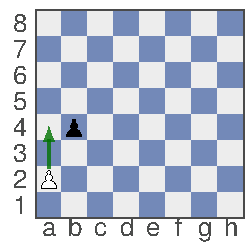
\includegraphics[width=\linewidth]{figures/ep_test.pdf}
\caption{\pos{W~a2 / B~b4}: $0$}
\end{subfigure}\hfill
\begin{subfigure}[t]{0.32\columnwidth}\centering
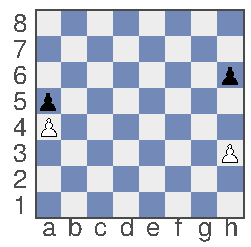
\includegraphics[width=\linewidth]{figures/zero_seam.pdf}
\caption{\pos{W~a4~h3 / \mbox{B~a5~h6}}: $0$}
\end{subfigure}\hfill
\begin{subfigure}[t]{0.32\columnwidth}\centering
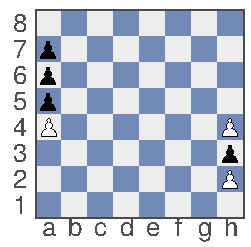
\includegraphics[width=\linewidth]{figures/tiny1_2025.pdf}
\caption{\pos{W~a4~h2~h4 / \mbox{B~a5~a6~a7~h3}}: $\tinyg{1}$}
\end{subfigure}
\caption{Basic positions. (a)~Ordinary board: after a2--a4 (arrow) the textbook test calls the a-pawn passed,
but b4$\times$a3 en passant removes it; under Definition~\ref{def:epaware} it is not passed. (b), (c)~Cylinder
(files a and h adjacent): a zero game and Tiny~1 that use the seam, in all nine settings. Positions of value
$1$, $2$, $\star$ and ${\uparrow}$ are in the supplementary material, Section~S1.}
\label{fig:basic}
\end{figure}

\begin{definition}[E.p.-aware passed pawn]\label{def:epaware}
A pawn is \emph{passed} if it passes the textbook test \emph{and} cannot be captured en passant on the
opponent's next move.
\end{definition}

One more white pawn makes the difference decisive. In \pos{W~a2~b3 / B~b4} black has no move, and the textbook
test lets white win at once with a2--a4. Under Definition~\ref{def:epaware}, every white move lets black capture
on a3, directly or en passant, and win the race that follows under the count rule, so the value is $0$. Across
the census of Section~\ref{sec:atlas} (at most six pawns, widths 1--4), the stricter test changes at least $18{,}137$ of the $231{,}071$ values,
$4{,}070$ of them in outcome \lab{C1} (Section~S1). The three race rules and three e.p.\ options
(textbook test, e.p.-aware test, e.p.\ off) give nine \emph{settings}. Values use the \emph{default setting}
(count rule, e.p.-aware test) unless stated.

\subsection{Components and the Cut Lemma}
A pawn changes file only by capturing onto a file where an enemy pawn stands (en passant included), so an empty
file stays empty forever and the pawns on either side of it never interact. Each block of neighboring occupied
files is a game of its own, a \emph{component}, and a position is the sum of its components; on the cylinder a
component is an arc or one \emph{ring} that uses every file.

\begin{theorem}[Cut lemma; \lab{P}, \lab{C2}]\label{thm:cut}
A pawn position on $\cyl{n}$ with at least one empty file has the same value as the position on
$\flatb{n-1}$ obtained by cutting the cylinder open along that file.
\end{theorem}

\begin{proof}
No pawn can move onto the empty file, so cutting the board there changes no legal move, no en passant right and
no passed-pawn test: the files beside the cut lose only a neighbor that stays empty forever.
\end{proof}

Hence values only a cylinder can make must come from rings (Section~\ref{sec:atlas}). A ring has no
empty file to separate a king group (Section~\ref{sec:kings-valid}), so ring values are pawn-model values only.

\section{Basic Positions on the Cylinder}\label{sec:basic}

The basic values of~\cite{Study2025} come from pawns alone. Each board in Fig.~\ref{fig:basic} leaves a file
empty, so by Theorem~\ref{thm:cut} its value is that of an ordinary-board position cut open along that
file~\cite{Elkies1996,WuYuLandry2010}, but the play crosses the seam. A move the opponent can answer with a
passed pawn loses and drops out~\cite{WinningWays,WuYuLandry2010}. The derivations of $1$, $2$, $\star$,
${\uparrow}$ and ${\Uparrow}\star$ are standard and are in Section~S1 of the supplementary material.

In Fig.~\ref{fig:basic}(b), if white goes first, it must play h3--h4, and black captures across the seam,
a5$\times$h4, with a passed pawn. If black goes first, h6--h5 is met by a4$\times$h5. Whoever moves first loses:
the value is $0$. Moving the white h-pawn back to h2 gives $1$, and moving the a-pawns up as well,
\pos{W~a5~h2 / B~a6~h7}, gives $2$, since black's h7--h5 is met by a5$\times$h6 en passant across the seam;
with e.p.\ off the value falls to the infinitesimal ${\Uparrow}\star$.

In Fig.~\ref{fig:basic}(c), white can take across the seam, h4$\times$a5, which leaves every pawn blocked: $0$.
White's h4--h5 drops out, since a6$\times$h5 wins for black. Black can only play a5$\times$h4; from there white
locks the a-file with a4--a5, leaving $0$, while black plays a6--a5 and keeps the spare move a7--a6, leaving
$-1$. So black's capture leads to $\game{0}{-1}=-\tfrac12\pm\tfrac12$, and $G=\tinyg{1}$, a positive
infinitesimal.

\section{Kings: The Tr\'ebuchet and When It Is Exact}\label{sec:kings}

In chess a player with no pawn move would move the king, or be stalemated, a draw. The tr\'ebuchet removes
stalemate: a side with no pawn move must move a king, and loses. We now ask when this gives the true chess result. Our king-and-pawn solver plays
real chess, with en passant, stalemate and any of the four promotions, but no fifty-move rule; an independent
reference solver, written from the rules alone, agrees with it on all $1{,}418{,}480$ positions of its test runs
\lab{C2}. Our solver's results below are \lab{C1} unless a second program or the Lichess
tablebase~\cite{LichessTB} confirms them.

\begin{figure}[!t]
\centering
\begin{subfigure}{0.32\columnwidth}
\centering
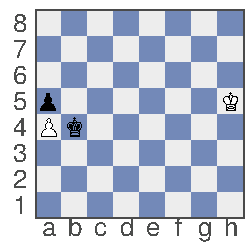
\includegraphics[width=\linewidth]{figures/trebuchet_2025.pdf}
\caption{\pos{W~Kh5~a4 / \mbox{B~Kb4~a5}}}
\label{fig:trebuchet_2025}
\end{subfigure}\hfill
\begin{subfigure}{0.32\columnwidth}
\centering
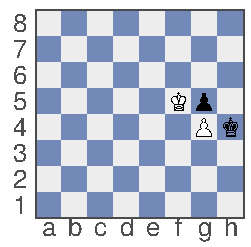
\includegraphics[width=\linewidth]{figures/trebuchet.pdf}
\caption{\pos{W~Kf5~g4 / \mbox{B~Kh4~g5}}}
\label{fig:trebuchet}
\end{subfigure}\hfill
\begin{subfigure}{0.32\columnwidth}
\centering
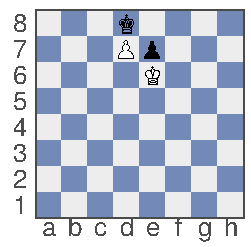
\includegraphics[width=\linewidth]{figures/kinggroup72.pdf}
\caption{\pos{W~Ke6~d7 / \mbox{B~Kd8~e7}}}
\label{fig:kinggroup72}
\end{subfigure}
\caption{King groups: (a) a tr\'ebuchet on the cylinder (files a and h adjacent) and (b) the tr\'ebuchet T
(ordinary board), both real mutual zugzwangs, $0$ when alone; (c) a king group from the 2025 study (cylinder;
Section~\ref{sec:sums}) that does not count as $0$: it draws with white to move, a zugzwang for black only.}
\label{fig:kings}
\end{figure}

In Fig.~\ref{fig:trebuchet_2025} only the kings can move. White to move must give up a4, since the only square
next to a4 that the king on h5 can move to, h4, is attacked by the a5 pawn across the seam; black to move loses
a5 in the same way. So this is a real mutual zugzwang that exists only because of the seam \lab{C2}.
Fig.~\ref{fig:trebuchet} shows the same idea on files f to h of the ordinary board; the Lichess tablebase
confirms that it is a mutual zugzwang \lab{C2}. We call this group T and place it beside every ordinary-board
pawn position in this paper.

\subsection{When Is the Frozen Tr\'ebuchet Exact?}\label{sec:kings-valid}

A \emph{king group} $Z$ is the two kings and some pawns on a block of files whose neighboring files, the
\emph{buffer}, hold no pawns; a \emph{decisive event} is a move in $Z$ or one creating a passed pawn.

\begin{theorem}[Validity of the convention; \lab{S}]\label{thm:validity}
Let a position consist of pawn components and a king group $Z$ with its buffer, let $X$, the position without $Z$, have no passed pawn, and suppose that before the
first decisive event:
\begin{enumerate}
\item[(V1)] outside $Z$ the legal chess moves are exactly the model's pawn moves, with the same results (en
  passant included); none gives check, nobody is in check, and the side to move has a legal move (one in $Z$
  counts);
\item[(V2)] in chess, the side that gets a passed pawn wins, and a race is won as the race rule says;
\item[(V3)] in chess, every move in $Z$ loses (it is \emph{decisively punished}).
\end{enumerate}
Then the chess result, with either side to move, is the outcome of $W(X)$, the pawn game that ends at the first
passed pawn (Section~\ref{sec:sums-hss}), without draws.
\end{theorem}

\begin{proof}[Proof sketch]
By (V3) neither side moves in $Z$ without losing, so until the first decisive event both play the pawn game;
by (V1) the side to move always has a legal move, a pawn move or a move in $Z$; the pawn game is finite, so some
decisive event occurs, and by (V2) and (V3) that event decides the chess game as it decides $W(X)$. The full
proof is in Section~S12.
\end{proof}

\begin{corollary}[\lab{S}]\label{cor:v4}
If also (V4) $X$ is hereditarily sum-safe (Definition~\ref{def:hss}) and satisfies condition (E) of
Theorem~\ref{thm:hss}, and $\BIG$ exceeds the number of moves either side can make, the chess result is
the outcome class of the components' $\pm\BIG$ value.
\end{corollary}

\begin{proof}
By Theorem~\ref{thm:validity} the chess result is the outcome of $W(X)$, and by Theorem~\ref{thm:hss} this is
the outcome of $S(X)$ (Section~\ref{sec:sums-hss}).
\end{proof}

Each condition can fail: a stalemate trap leaves the loser without a move (V1), a passed pawn does not win its
race (V2), a king walks over to the pawns or, in Fig.~\ref{fig:kinggroup72}, white's king moves go unpunished
(V3), and a $+\BIG$ cancels a $-\BIG$ (V4). For (V3) there is a local test: a move in $Z$ has a
\emph{certificate of horizon $h$} if, with only $Z$ on the board, the punisher promotes or mates within $h$
moves of its reply, no defender pawn outside $Z$ is that fast, and no stalemate comes first. In the \emph{promotion game} (the first
promotion wins) such a move loses for its mover \lab{S}; in chess even wider margins can fail. The exact clauses and the proof are in Section~S12; a local test for (V2)
and the loopy games of kings with spare moves are in Section~S2.

\subsection{How Often Does the Convention Fail?}\label{sec:kings-sweep}

We solved, with the kings played out, every component with at most two pawns a side beside a tr\'ebuchet on
boards with six ranks (one file of the six-file cylinder and of the five-file ordinary board, files d and e of
the seven-file cylinder; queen promotions only, at most two). Of these, $500$ start without a race and have a
determined result. Under the textbook test, $159$ of the $500$ get the wrong outcome \lab{C1}: $107$ through
the kings alone, $18$ through en passant and $34$ because a passed pawn does not win its race. The e.p.-aware
test repairs the $18$ e.p.\ failures, but the kings undo $13$ of these repairs. In each race failure a blocked
enemy pawn steps level with its blocker and promotes first. Ending the game only at a passer
that wins the race by the square rule removes all $52$ convention failures with frozen kings; with real kings
$31$ stay repaired, which leaves $128$ mismatches, all from the kings \lab{C1}. The rule is not sound on every
board (Section~S16). Of the $2{,}154$ $8\times8$ positions beside a tr\'ebuchet whose real results we know, $105$ are
draws; in the other $2{,}049$ the model names the winner in $92.5\%$, against $83\%$ and $84\%$ under the mover
and opponent rules \lab{C1} (Section~S2).

\section{Sums, Temperature and the Puzzles Revisited}\label{sec:sums}

Most endgames are sums of components. Two principles guide play in them. By \emph{number avoidance}, in a sum of
numbers and games that are not numbers, a player who can win can do so without moving in a
number~\cite{WinningWays,Siegel2013}. By the heuristic of the \emph{hottest move}, one moves in the component of
highest temperature: for a switch $\game{x}{y}$ between numbers $x>y$, the temperature $(x-y)/2$ is what each
side gains by moving there first.

\subsection{The Puzzles Revisited}

Table~\ref{tab:puzzles} compares the values first claimed for three puzzles of~\cite{Study2025} with the exact
ones: the earlier walk-throughs pick the right winners, but not always the right values. In Puzzle~1, black's
h6$\times$a5 across the seam leaves $\star$, so the h/a component is hot, not the number $1$. The
pawns of Puzzle~2 form an infinitesimal with mean $0$, and its king group (Fig.~\ref{fig:kinggroup72}) is a
zugzwang for black only, on the ordinary board \lab{C2} (our solver and the Lichess tablebase) and on the
cylinder \lab{C1}, so the real result of this ten-man position is open. Puzzle~3 is illegal as drawn; on files c and d its value is $\tinyg{1}$, and the legal copy
one rank up, \pos{W c2 c4 d4 / B c3 d5 d6 d7}, has the same value (Section~S3 shows the puzzles).

\begin{table}[!t]
\centering
\caption{Puzzles of the 2025 Study: Claimed and Exact Values \lab{C2}}
\label{tab:puzzles}
\begin{tabular}{@{}lll@{}}
\toprule
Part & Claimed~\cite{Study2025} & Exact \\
\midrule
1: c-file & $\pm1$ & $\pm1$ \\
1: f-file & $\game{\game{2}{1}}{0}$ & the same (mean $3/4$) \\
1: files h, a & $1$ & $\game{+\BIG}{\star}$ (hot) \\
1: total & $1\pm1+\game{\game{2}{1}}{0}$ & white wins either way \\
2: pawns & $\pm1$ & infinitesimal, mean $0$ \\
2: kings & $0$ & not mutual \\
3: files c, d & $1$ & $\tinyg{1}$ \\
3: total & $2$ & $+\BIG$ before any move \\
\bottomrule
\end{tabular}
\end{table}

\subsection{When Is the Sum Model Right?}\label{sec:sums-hss}

In chess the first passed pawn ends the game; in a sum, a component with a passed pawn becomes $\pm\BIG$ and
play goes on elsewhere, so a $+\BIG$ can cancel a $-\BIG$. In $\game{\BIG}{0}+\game{0}{-\BIG}$ the first player
makes a passed pawn and wins the chess game, but the sum is $0$ for every $\BIG$, since the second player
answers in the other component \lab{P}. We write $W(X)$ for the whole-board game of a pawn position $X$, which
ends at the first passed pawn, and $S(X)$ for its sum model, which after every move re-splits the pawns into
components along empty files (one ring if no file is empty), replaces a component in which a side has a passed
pawn by $\pm\BIG$ (by the race rule if both have one) and adds the components up. We call $W(X)$ a $\nim{k}$ when
$W(X)+\nim{h}$ has the outcome of $\nim{k}+\nim{h}$ for every heap $h$; our scans and the wall proofs test
exactly this.

\begin{definition}[Hereditary sum safety]\label{def:hss}
A component carries a \emph{threat} for a side if a position reachable from it gives that side a passed pawn. A
position $X$ is \emph{hereditarily sum-safe} (HSS) if no position reachable from $X$ by moves of either side,
in any order, before the first passed pawn, $X$ included, has two components with threats for opposite sides.
\end{definition}

\begin{theorem}[Sum safety; \lab{S}]\label{thm:hss}
Suppose that $X$ is HSS, that no position reachable from $X$ with two or more components has a usable en
passant right (condition (E)), and that $\BIG$ exceeds the number of moves either side can make. Then $S(X)$ and
$W(X)$ have the same outcome.
\end{theorem}

\begin{proof}[Proof sketch]
The models differ only after a passed pawn appears, say for white. By HSS no other component can then give black
one, so black runs out of moves before white's $+\BIG$ does. The full proof, by induction with (E), is in
Section~S12 of the supplementary material.
\end{proof}

In a random sample of $1{,}500$ positions, all $1{,}297$ HSS ones agree \lab{C1}, and with $\BIG=256$ the move
bound always holds on boards up to $8\times8$. HSS cannot be dropped (Proposition~\ref{prop:sumcounter}); without
(E) the decomposition already fails in the pure pawn game, without the passed-pawn rule \lab{C1} (Section~S3).

\begin{proposition}[\lab{C2}]\label{prop:sumcounter}
A test of the top-level components alone is not enough: on $\cyl{8}$ with en passant off, $X=$\,\pos{W b2 d4 g3
h5 / B a7 c7 f7 g4} is a single component, spanning files f to d across the seam, so such a test passes it; yet
$S(X)$ is a black win whoever starts and $W(X)$ a first-player win. Moreover $X$ is not HSS: components with
opposite threats appear later in its tree, so Theorem~\ref{thm:hss} does not apply.
\end{proposition}

\emph{Two models.} Our CGT engine computes $S$, as Elkies does~\cite{Elkies1996}, and the independent
whole-board solver $W$. They agree on every headline value: the $1/8$ and $\upsec\star$ in all nine settings,
and the seven-pawn $\nim{2}$ in the default setting. Elsewhere they can differ, even in outcome (Section~S3);
there we name the model we mean.
% SLOT: real-king sum test

\section{The Atlas: What Only the Cylinder Can Do}\label{sec:atlas}

We computed two collections of positions with every pawn on ranks 2--7, at least one pawn per side and no
passed pawn. \emph{The atlas} holds every such position with at most five pawns on
$\cyl{3},\dots,\cyl{8}$ and $\flatb{3},\dots,\flatb{8}$, up to symmetry: $1{,}223{,}689$ positions
\lab{C1}. An independent minimax program confirms their textbook winners for all
$12{,}568$ rings and $4{,}000$ random ordinary components. \emph{The census} holds every such position
with at most six pawns on $\flatb{1},\dots,\flatb{4}$, up to translation and mirror image:
$231{,}071$ records standing for $459{,}443$ positions.

Under the textbook test, the atlas values free of $\BIG$ include just two nimbers: $\star$, and one
$\nim{2}$, the textbook candidate of Section~\ref{sec:star2}, which the e.p.-aware test removes. They also
include several ups and fractions with denominator at most $4$; apart from $\pm\BIG$ the highest temperature is
$3$ \lab{C1} (Section~S4). A value that occurs on a cylinder but on no ordinary board is \emph{cylinder-only}. By the cut
lemma (Theorem~\ref{thm:cut}) it comes from a ring, which on $n$ files needs $n$ pawns.

\begin{proposition}[\lab{C1}]\label{prop:cylonly}
Under the textbook test, $53$ atlas values free of $\BIG$ are cylinder-only: $40$ from $3$-file rings and
$13$ from $4$-file rings; the five-pawn rings on $\cyl{5}$ give none. No atlas value occurs only on ordinary boards.
\end{proposition}

For example, on $\cyl{3}$, white a2, b4 against black b7, c6 is $3/4$. These values are not robust: the $3$-file ones depend on the race rule ($3/4$ becomes $0$ under the mover rule), the $4$-file ones on
the e.p.\ option. We compared all nine settings only for positions with at most four pawns; among them no value
is cylinder-only in all nine \lab{C1}. Section~S4 of the supplementary material shows these positions.

\section{Elkies' Small Values}\label{sec:targets}

Elkies~\cite{Elkies1996} found fractions, ups and tinies in chess endgames on the ordinary board. We searched
the census (Section~\ref{sec:atlas}) for smaller values of these kinds: $1/8$, $1/16$ and $1/32$;
\emph{up-second} $\upsec=\game{0}{{\downarrow}\star}$, positive but smaller than ${\uparrow}$, and
$\upsec\star=\game{0,\star}{{\downarrow}}$; and the \emph{tinies} $\tinyg{x}=\ggame{0}{0\mid -x}$ (a number $x$).
Table~\ref{tab:targets} counts them under both passed-pawn tests; under the e.p.-aware test $1/32$
disappears. We do not claim these kinds of value as new; what is new is $10$-man positions with a legal pawn
history, checked in all nine settings (Tiny~1 in the six with en passant on).

\begin{table}[!t]
\caption{Elkies' Small Values in the Census}
\label{tab:targets}
\centering
\begin{tabular}{@{}llcc@{}}
\toprule
Value & Form & Textbook & E.p.-aware \\
\midrule
$1/8$ & $\game{0}{1/4}$ & $13$ & $9$ \\
$1/16$ & $\game{0}{1/8}$ & $3$ & $2$ \\
$1/32$ & $\game{0}{1/16}$ & $1$ & $0$ \\
$\upsec$ & $\game{0}{{\downarrow}\star}$ & $5$ & $2$ \\
$\upsec\star$ & $\game{0,\star}{{\downarrow}}$ & $10$ & $10$ \\
$\tinyg{1}$ & $\ggame{0}{0\mid -1}$ & $13$ & $16$ \\
\bottomrule
\end{tabular}

\smallskip
\parbox{\columnwidth}{\footnotesize Positions of each exact value in the census (count rule); no census position
is $\tinyg{x}$ with $x\notin\mathbb{Z}$. Textbook column: an independent C solver confirmed each identity
(position minus target $=0$) \lab{C2}. E.p.-aware column: \lab{C1}.}
\end{table}

\begin{figure}[!t]
\centering
\begin{subfigure}[b]{0.32\columnwidth}\centering
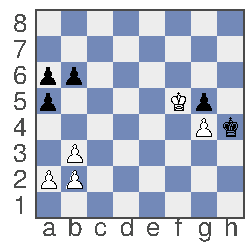
\includegraphics[width=\linewidth]{figures/eighth.pdf}
\caption{}
\end{subfigure}\hfill
\begin{subfigure}[b]{0.32\columnwidth}\centering
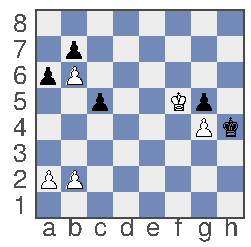
\includegraphics[width=\linewidth]{figures/upsecstar.pdf}
\caption{}
\end{subfigure}\hfill
\begin{subfigure}[b]{0.32\columnwidth}\centering
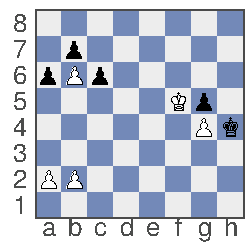
\includegraphics[width=\linewidth]{figures/tiny1.pdf}
\caption{}
\end{subfigure}
\caption{Elkies' small values beside T (Fig.~\ref{fig:trebuchet}), each a 10-man position with a legal pawn
history (ordinary board). (a)~$1/8$: \pos{W a2 b2 b3 / B a5 a6 b6}. (b)~$\upsec\star$: \pos{W a2 b2 b6 / B a6 b7 c5}.
(c)~$\tinyg{1}$: \pos{W a2 b2 b6 / B a6 b7 c6}.}
\label{fig:eighth}
\end{figure}

\begin{theorem}[\lab{C2}]\label{thm:eighth}
In the pawn model, white a2, b2, b3 against black a5, a6, b6 has value exactly $1/8$ in all nine settings
and for every assignment of outcomes to its race positions (Section~\ref{sec:rules}).
\end{theorem}

In Fig.~\ref{fig:eighth}(a), white's a2--a4 locks the a-file and leaves $0$; a2--a3 reaches only $\star$ and is
reversible, and b3--b4 is bad. Black's b6--b5 leaves $1/4$, and a5--a4 is bad. Thus $G=\game{0}{1/4}=1/8$. This
structure arises from the starting position by c2$\times$b3, a7--a5, b7$\times$a6 and c7$\times$b6. The checks
ran on its mirror image (Section~S5).

White a2, b2, b6 against black a6, b7, c5 (Fig.~\ref{fig:eighth}(b)) is $\game{0,\star}{{\downarrow}}=\upsec\star$
in all nine settings \lab{C2}: white's a2--a4 and a2--a3 leave $0$ and $\star$, black's a6--a5 leaves
${\downarrow}$. With the c-pawn on c6 (Fig.~\ref{fig:eighth}(c)), white's a2--a3 leaves $0$ and black's a6--a5
leaves $\game{0}{-1}$, which dominates c6--c5, so $G=\tinyg{1}$ under every race rule with en passant on
(textbook test \lab{C2}, e.p.-aware test \lab{C1}); with e.p.\ off it is ${\uparrow}$. Unlike
Fig.~\ref{fig:basic}(c), it needs no seam. Both structures arise from the starting position by c2$\times$b3,
b3--b4--b5--b6, a7--a6 and c7--c5 (c7--c6 for Tiny~1). A textbook-test $1/8$ and $\upsec$ in the census fail under the e.p.-aware test (Section~S5), so we state
these values for all nine settings.

\section{The \texorpdfstring{$\nim{2}$}{*2} Question}\label{sec:star2}

\subsection{The Textbook Candidate}

\begin{figure}[!t]
\centering
\begin{subfigure}{0.32\columnwidth}\centering
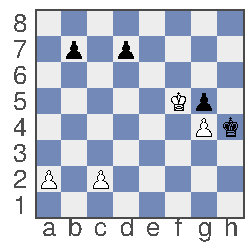
\includegraphics[width=\linewidth]{figures/star2_textbook.pdf}
\caption{Candidate}\label{fig:star2_textbook}
\end{subfigure}\hfill
\begin{subfigure}{0.32\columnwidth}\centering
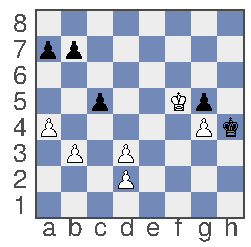
\includegraphics[width=\linewidth]{figures/star2_seven_a.pdf}
\caption{Position A}\label{fig:star2_seven_a}
\end{subfigure}\hfill
\begin{subfigure}{0.32\columnwidth}\centering
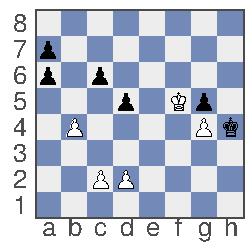
\includegraphics[width=\linewidth]{figures/star2_seven_b.pdf}
\caption{Position B}\label{fig:star2_seven_b}
\end{subfigure}
\caption{Positions of the $\nim{2}$ question beside T (Fig.~\ref{fig:trebuchet}; ordinary board). (a)~Candidate:
$\nim{2}$ under the textbook test, $\game{2\pm1}{-2\pm1}$ under the e.p.-aware test. (b)~Position A and
(c)~position B: $\nim{2}$ in the default setting.}
\label{fig:star2}
\end{figure}

The candidate \pos{W a2 c2 / B b7 d7} (Fig.~\ref{fig:star2_textbook}) is, under the count rule with the
textbook test, the only $\nim{k}$ with $k\ge2$ in the census: a2--a4 and c2--c4 leave $\star$ and $0$, and by
symmetry black's d7--d5 and b7--b5 do the same, so $G=\game{0,\star}{0,\star}=\nim{2}$. Its weak point is
black's b7--b5 and b5--b4: the textbook test then scores a2--a4 as $+\BIG$, but black takes b4$\times$a3 en
passant (Fig.~\ref{fig:basic}(a)). Under the e.p.-aware test \pos{W a2 c2 / B b4 d7} is worth $-3$, b7--b5 is
worth $-2\pm1$ and, by symmetry, c2--c4 is worth $2\pm1$; the other moves are dominated or reversible, so
$G=\game{2\pm1}{-2\pm1}$, a hot game with mean $0$ and temperature $2$ \lab{C2} (Section~S6 gives the details).

\subsection{No \texorpdfstring{$\nim{2}$}{*2} With Six Pawns or Fewer}

\begin{theorem}[Census; \lab{C2}]\label{thm:census}
In the census of Section~\ref{sec:atlas}, in the default setting, no position has value $\nim{k}$ with
$k\ge2$; the census has $6{,}724$ zeros and $4{,}042$ stars.
\end{theorem}

Our CGT engine and an independent C solver agree on every record, and the independent whole-board solver
finds no $\nim{k}$ with $2\le k\le 292$ among $793{,}299$ labeled placements on widths 1--4; every position in
scope has birthday at most $292$. Under the textbook test the census has $6{,}470$ zeros, $3{,}891$ stars and the candidate.

\subsection{\texorpdfstring{$\nim{2}$}{*2} With Seven Pawns}

\begin{theorem}[$\nim{2}$ with seven pawns; \lab{C2}]\label{thm:star2seven}
In the default setting, position~A, \pos{W a4 b3 d2 d3 / B a7 b7 c5}, and position~B,
\pos{W b4 c2 d2 / B a6 a7 c6 d5}, on files a--d of the ordinary board, have value $\nim{2}$. Neither is $\nim{2}$
with e.p.\ off or under the opponent rule.
\end{theorem}

Both fit beside T, and their pawns can arise in a game (Section~S6). In position A (Fig.~\ref{fig:star2_seven_a}), if white moves first, a4--a5 leaves $0$. The move d3--d4 attacks
c5; every black reply except c5$\times$d4 loses at once, and after c5$\times$d4 white continues b3--b4 to
$\star$, so the reversible move d3--d4 counts as a move to $\star$. White's third move, b3--b4, loses to
c5$\times$b4. If black moves first, a7--a5 leaves $0$ and b7--b6 leaves $\star$. Black's other moves are
reversible: after a7--a6 and b7--b5 white has replies worth $2$ and $3$, both at least $G$; and c5--c4
lets d3$\times$c4 free white's d2 pawn for $+\BIG$. Thus $G=\game{0,\star}{0,\star}=\nim{2}$. Position B is A
with the colors reversed and the files mirrored, and its analysis matches move for move (Section~S6).

\begin{table}[!t]
\centering
\caption{Values of the Candidate and of Positions A and B in the Model Settings}
\label{tab:star2_settings}
\footnotesize
\setlength{\tabcolsep}{4pt}
\begin{tabular}{@{}lccc@{}}
\toprule
Race rule, passed-pawn test & Candidate & A & B\\
\midrule
count, e.p.-aware & $\game{2\pm1}{-2\pm1}$ & $\nim{2}$ & $\nim{2}$\\
mover, e.p.-aware & $\game{2\pm1}{-2\pm1}$ & $\nim{2}$ & $\nim{2}$\\
count or mover, textbook & $\nim{2}$ & $\nim{2}$ & $\nim{2}$\\
count or mover, e.p.\ off & $\nim{2}$ & not $\nim{2}$ & not $\nim{2}$\\
opponent, any e.p.\ option & $0$ & not $\nim{2}$ & not $\nim{2}$\\
\bottomrule
\end{tabular}
\end{table}

In Table~\ref{tab:star2_settings} (e.p.\ on unless stated) every entry is \lab{C2}; for A and B, three
programs agree on each. The candidate needs the textbook test but survives e.p.\ off; A and B need en passant
but not the textbook test.

\subsection{Counts}\label{sec:star2-five}

On ordinary boards of width at most four, in the default setting, two $\nim{2}$ positions, A and B, have seven
pawns and four have eight; one exhaustive scan of $5{,}503{,}282$ root positions gives these counts \lab{C1},
and our engine re-checked every one \lab{C2}. With Theorem~\ref{thm:census}, seven is the least number of pawns
in a $\nim{2}$ on these boards \lab{C2}. A whole-board scan of every position with at most seven
pawns on up to nine files extends this to ordinary boards of any width (Section~S6): it finds no $\nim{k}$ with $k\ge2$ with six pawns or
fewer, and the only seven-pawn $\nim{2}$ are A and B \lab{C2}; Section~S6 gives the counts on five files.

\subsection{Rings and Higher Nimbers}\label{sec:star2-rings}

\begin{figure}[!t]
\centering
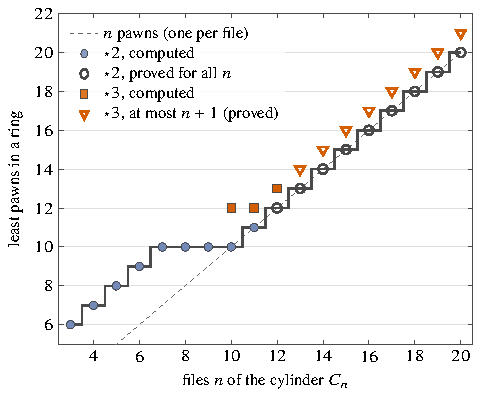
\includegraphics{figures/f2_least_pawns.pdf}
\caption{Least number of pawns in a ring of value $\nim{2}$ (steps) and $\nim{3}$ on $\cyl{n}$, in the default
setting. Filled markers are computed minima (\lab{C2} for $\nim{2}$, \lab{C1} for $\nim{3}$), open ones proved for all
$n$ as whole-board games \lab{S}; open triangles are upper bounds. The dashed line is one pawn per file. $\nim{3}$ is plotted from $n=10$;
ten-pawn $\nim{3}$ rings also exist on $\cyl{7}$ and $\cyl{8}$.}
\label{fig:least}
\end{figure}

Fig.~\ref{fig:least} gives the least ring $\nim{2}$ and $\nim{3}$ on each cylinder; Section~S6 lists example rings, counts and checks for every $n$. The first ring $\nim{2}$ on
$\cyl{n}$ has $n+3$ pawns for $n=3,\dots,7$ \lab{C2}, among them the six-pawn \pos{W a2 a3 b2 / B b7 c6 c7} on
$\cyl{3}$, one pawn fewer than any ordinary board of width at most four allows; it needs two en passant
captures, and with e.p.\ off it is $0$ \lab{C2}. On $\cyl{8}$ and $\cyl{9}$ ten is again the least \lab{C2}.
From $\cyl{10}$ on, one pawn per file, the least a ring can have, suffices: \pos{W b2 d2 e3 h3 j5 / B a4 c6 f6
g7 i7} on $\cyl{10}$ (the ring $M_{10}$ of Fig.~\ref{fig:ring}) and \pos{W c5 e3 h3 i2 k2 / B a4 b7 d7 f7 g6 j6}
on $\cyl{11}$ are $\nim{2}$ \lab{C2}.

For proofs we use \emph{walls}: runs of files with one pawn each, alternating in color, the black pawn two
ranks above the white (B4, W2: a black pawn on rank 4, a white one on rank 2). If a wall pawn moves, its neighbor
captures it and gets a passed pawn, so wall moves lose; with them deleted, inserting a pair of wall files leaves
the \emph{reduced game}, played in a window of five or six files, unchanged. As a whole-board game this gives a
ring $\nim{2}$ with $n+3$ pawns on every $\cyl{n}$ with $n\ge5$ \lab{S}, checked by two programs for $n<17$
\lab{C2}, and as sums of components our engine confirms it only to $n=12$ \lab{C1}. The same argument proves the
two $n$-pawn families above $\nim{2}$ as whole-board games for every $n\ge10$ \lab{S}; as sums of
components they are $\nim{2}$ on $\cyl{10}$ and $\cyl{11}$ \lab{C1}.

A $\nim{3}$ lies just beyond these scans, as a single component with nine pawns: B with a white a2 and a black a4
added, \pos{W a2 b4 c2 d2 / B a4 a6 a7 c6 d5}, is $\nim{3}$ on four files \lab{C2}. In the whole-board game no
position with eight pawns or fewer on up to eight files, ordinary or cylinder, is $\nim{3}$ \lab{C1}. On
$\cyl{7}$ eight ten-pawn rings are $\nim{3}$ \lab{C2}. Wall insertion gives a whole-board $\nim{3}$ with $n+2$
pawns on every $\cyl{n}$ with even $n\ge8$ and odd $n\ge11$, and with $n+1$ pawns on every $\cyl{n}$ with
$n\ge12$ \lab{S}. Height matters: on boards of three to five files, seven ranks give a $\nim{2}$ with four
pawns, \pos{W a2 c2 / B c3 b6}, and a $\nim{3}$ with six; six ranks give a $\nim{2}$ and five give none
\lab{C2}. But no $\nim{4}$ has turned up:
none of the $134{,}920{,}191$ one-component ten-pawn positions on five files has a nimber above $\nim{3}$, nor has any of about $24$ million rings or of $1.8$ billion positions on these narrow boards with $5$ to $12$
ranks \lab{C1} (Section~S6).

\emph{M\"obius strip.} With the first and last files joined and the ranks reversed, a pawn that captures across
the seam lands on the mirrored rank and turns round. The least ring $\nim{2}$ then has $6, 8, 6, 8, 8, 8$ pawns
for $n=3,\dots,8$ files, against $6, 7, 8, 9, 10, 10$ on the cylinder, and $10, 10, 11$ for $n=9,10,11$ on both
\lab{C2}. One pawn per file is enough on eight files, not on nine, and from ten on in two families that stay
$\nim{2}$ up to $32$ files \lab{C1}. Nine pawns give a $\nim{3}$ on five and on six files \lab{C2}.

In the model, then, the $\nim{2}$ question has a positive answer on the ordinary $8\times8$ board: four files
and seven pawns beside T suffice, while Elkies' higher nimbers need larger boards~\cite{Elkies2002}.

\section{From the Model to Real Chess}\label{sec:real}

To test a model value, we keep its tree of pawn moves and replace only the leaves by real results, from the
Lichess tablebase~\cite{LichessTB} up to seven men and beyond from search and our king-and-pawn solver.

\begin{definition}[Real-chess oracle value]\label{def:oracle}
Let $X$ be a pawn component on the ordinary board beside T. An \emph{end position} of its model tree is a
position where a line of play first reaches a passed pawn; its two \emph{sides} are white to move and black to
move. Replace each end position by $+\BIG$ if white wins it in real chess with either side to move, by $-\BIG$
if black does, by $\game{+\BIG}{-\BIG}$ if the side to move wins, and by $0$ if the side to move loses. If a side
is drawn, the \emph{draw treatment} counts that draw as a win for black, as a win for white, or as worth $0$; in
the last case the end position is $\game{\BIG r_W}{\BIG r_B}$, where $r_W,r_B\in\{-1,0,1\}$ are white's results
with white and with black to move. The canonical value of the resulting tree is the \emph{oracle value} $O(X)$.
\end{definition}

\begin{lemma}[Sandwich; \lab{P}]\label{lem:sandwich}
Replace every end position whose real-chess value is not known by $-2\BIG$ (for $O^-$) or by $+2\BIG$ (for
$O^+$), and keep every known one, scored as in Definition~\ref{def:oracle} under the chosen draw treatment. Then
$O^-\le O(X)\le O^+$ whatever the unknown results; if $O^-=O^+$, $O(X)$ is certified.
\end{lemma}
\begin{proof}
Every leaf lies between $-2\BIG$ and $2\BIG$, and raising an option never lowers a
game~\cite{Siegel2013}; induct from the leaves.
\end{proof}

\subsection{The Textbook Candidate in Real Chess}\label{sec:real-cand}

The tree is built under either passed-pawn test: the \emph{textbook tree} or the \emph{e.p.-aware tree}.

\begin{theorem}[Candidate in real chess; \lab{C1}]\label{thm:oracle-cand}
For the candidate \pos{W a2 c2 / B b7 d7} beside T (Fig.~\ref{fig:star2_textbook}):
\begin{enumerate}
\item[(a)] In chess the side to move wins; with black to move only 1\ldots~b5 wins; with white to
  move 1.~c4 wins, 1.~a3, 1.~c3 and all king moves lose, and 1.~a4 is unresolved \lab{C2}.
\item[(b)] In the e.p.-aware tree, for every draw treatment, $O$ has left stop $\ge1$ and right stop $\le-1$, so
  it is not $0$ or $\nim{2}$.
\item[(c)] With draws as wins for black, $O=\game{2\pm1}{-2\pm1}$ in both trees.
\end{enumerate}
\end{theorem}

Real chess thus agrees with $\nim{2}$ on the outcome and on every winning first move resolved so far, but not on
the value: in the e.p.-aware tree, which matches chess, $O$ is hot under every draw treatment, so the candidate's
$\nim{2}$ is a feature of the textbook test, not of chess. In the textbook tree, $\nim{2}$ is excluded
if draws count as wins for either side \lab{C1}, and undecided if draws count $0$. A second candidate, \pos{W a3 b3 c2 / B b5 b7 c6},
$\nim{2}$ under the opponent rule with en passant on, has a positive oracle value under every draw treatment
\lab{C1}; the other non-default $\nim{2}$ positions are open (Section~S7).

\subsection{Towards a Real-Chess \texorpdfstring{$1/8$}{1/8}}\label{sec:real-eighth}

The $1/8$ position of Section~\ref{sec:targets} has $10$ men. Its e.p.-aware tree has $302$ end-position sides
with at most seven men, all resolved by the tablebase: in $290$ only one side has a passed pawn, of which $283$
agree with the model, $5$ disagree and $2$ are draws. A search for the larger end positions that decide the value
leaves, after one eight-man result against the model, one eight-man position and three of nine men; our
king-and-pawn solver (queen promotions only) shows that all four agree with the model on both sides. The hardest,
black to move in \pos{W b2 b5 / B a5 b4}, needed $6.1\times10^{10}$ states in $15.6$~h (Section~S7).

\begin{proposition}[A tablebase-backed oracle value of $1/8$; \lab{C1}]\label{prop:eighth-real}
For the $1/8$ position, with queen promotions only in our solver, $O=1/8$, whatever the open end positions do.
\end{proposition}

It assumes frozen kings; the full-chess value is open. For
$\upsec\star$ and $\tinyg{1}$ the lower bounds already equal the target values, with $10$ and $12$ end positions
of $9$ or $10$ men still open \lab{C1}. For positions A and B ($11$ men beside T) the deciding end positions with
$8$ men agree with the model \lab{C2}, but those with $9$ to $11$ men are unsolved, so their $\nim{2}$ is a model
value.

\section{Mating Without Corners: Tablebases}\label{sec:tb}

Which material can force mate without corners? We computed the tablebases of eight pawnless endings,
king and one or two pieces against the bare king, on the ordinary board, on the cylinder and on the torus, where
ranks 1 and 8 are joined as well. Chess on these boards is an old variant~\cite{Pritchard}, and other changes to the rules of chess have been studied with
self-play engines~\cite{Tomasev2022}. Prose sources say
that king and rook cannot force mate on the cylinder, nor king and queen on the torus~\cite{WikiCylinder,HGMCylinder};
we confirm the torus claim, but the rook mates from 2.80\% of cylinder positions. We know of no earlier tablebase
for them.

\emph{Rules and verification.} Pieces wrap round each glued edge; there is no castling and no fifty-move rule,
and stalemate and bare kings are draws. A position is legal when the kings are not adjacent, across the seams
included, and the side not to move is not in check. Two retrograde solvers~\cite{Thompson1986}, written independently, agree on
every position of all 24 tables, about 607 million values with either side to move \lab{C2}; on the ordinary
board both reproduce the known longest mates.

\begin{table}[!t]
\centering
\caption{Pawnless Endings Against the Bare King on the Ordinary Board, Cylinder and Torus: Share Won With
White to Move and Longest Mate \lab{C2}}
\label{tab:tb}
\footnotesize
\setlength{\tabcolsep}{4.5pt}
\begin{tabular}{@{}lrrrrrr@{}}
\toprule
& \multicolumn{2}{c}{Ordinary} & \multicolumn{2}{c}{Cylinder} & \multicolumn{2}{c}{Torus} \\
\cmidrule(lr){2-3}\cmidrule(lr){4-5}\cmidrule(l){6-7}
Material & Won (\%) & Mate & Won (\%) & Mate & Won (\%) & Mate \\
\midrule
KQK  & 100    & 10 & 100    & 10 & 0      & --- \\
KRK  & 100    & 16 & 2.80   & 3  & 0      & --- \\
KBBK & 99.98  & 19 & 100    & 14 & 0      & --- \\
KBNK & 99.51  & 33 & 0.0245 & 2  & 0      & --- \\
KNNK & 0.0107 & 1  & 0.0077 & 1  & 0      & --- \\
KRBK & 100    & 16 & 99.74  & 13 & 0.0218 & 1   \\
KRRK & 100    & 7  & 100    & 8  & 100    & 7   \\
KQRK & 100    & 6  & 100    & 5  & 100    & 5   \\
\bottomrule
\end{tabular}

\smallskip
\parbox{\columnwidth}{\footnotesize Mate: longest forced mate in moves; ---: no position is won. KBBK has
the bishops on opposite colors. KRK is king and rook against king, and so on.}
\end{table}

\emph{KRK and KBNK rarely force mate on the cylinder} (Table~\ref{tab:tb}; White to move throughout), while KQK wins every position, as
quickly as on the ordinary board. The rook wins only 2.80\% of the positions, all from mating nets already in place, such as Ka3, Rb2 against Ka1:
1.~Rb3 Kh1 2.~Rg3 Ka1 3.~Rg1\#, where the rook covers h1 and the white king h2, the flight squares across the
seam. The standard bishop-and-knight mate needs a corner of the bishop's color, and the cylinder has none.

\emph{Bishops on opposite colors win every position on the cylinder}, and faster than on the ordinary board,
although the bishop pair is said not to mate there~\cite{HGMCylinder}: every diagonal winds round from the first
rank to the eighth. The longest line ends in Ke6, Be1, Bf1 against Ke8: the bishop on f1 checks along
f1--h3--a4--e8, across the seam, and the bishop on e1 covers d8 and f8.

\emph{On the torus, of the eight endings, only KRRK and KQRK force mate}, and they win from every position;
KRBK wins only where a mate in one is already set up. KRK wins everywhere on the M\"obius strip (files a and h
joined, ranks reversed), but only $0.66\%$ on the Klein bottle \lab{C2}.

\subsection{King and Pawn Against King}\label{sec:kpk}

We solved every legal KPK position on the $8\times8$ ordinary board and cylinder twice, with our king-and-pawn
solver (all four promotions) and with a separately written KPK solver (queen promotion only). They agree on all
326,640 cylinder positions and differ on exactly 6 ordinary-board positions, where only a rook promotion wins,
such as Ka4, Pb7 against Ka6 \lab{C2}. The rook-pawn draw disappears: Ka6, Pa5 against Ka8 is a white win on the
cylinder whoever moves, since shifting every man four files gives the textbook win Ke6, Pe5 against Ke8. Of the
positions legal on both boards, 16,538 ordinary-board draws become cylinder wins, and 15,930 wins become draws,
since a king on the h-file stands beside an a-pawn. Zugzwang, the engine of the tr\'ebuchet, is more common on the cylinder: 216 reciprocal zugzwangs (white
to move draws, black to move loses) against 160 on the ordinary board \lab{C2}. Section~S8 gives the counts, other widths $\cyl{3}$ to $\cyl{10}$ and KPKP.

\section{Dawson's Chess on the Cylinder}\label{sec:dawson}

On a cylinder every file is alike, and the first move opens the ring of files into an ordinary strip. The
earlier study~\cite{Study2025} used this idea on Dawson's chess but stated the game incorrectly; we
redo it.



\emph{Rules.} Dawson's chess~\cite{Dawson1935} is played on a $3\times n$ board
(Section~S9 shows the boards) with white pawns on rank~1, black pawns on rank~3 and rank~2 empty. Pawns move
and capture as in chess, captures are compulsory, and no pawn can double-step or promote. The last player to
move wins; in the mis\`ere form that Dawson posed, the last player loses.

Call a file \emph{untouched} if both its pawns stand on their starting squares. If white plays c1--c2 with the
b- and d-files untouched, the captures b3$\times$c2, d1$\times$c2, d3$\times$c2 and b1$\times$c2 are forced
(up to the choice of side), and leave black to move with the b- and d-files empty and the c-file blocked for
good. At the end of a row the push takes three plies and empties its one neighbor; a push with no untouched
neighbor is blocked. Counting each forced sequence as one move, strips separated by empty files never interact,
and the game is impartial: a strip of $n$ untouched files is the octal game
$\mathbf{0.137}$~\cite{GuySmith1956,WinningWays}, in which a move removes a file and its untouched neighbors. Its
Grundy values are $g(0)=0$, $g(1)=1$ and, for $n\ge2$,
\begin{equation}\label{eq:dawson}
g(n)=\operatorname{mex}\bigl(\{g(n-2)\}\cup\{g(a)\oplus g(b) : a+b=n-3\}\bigr),
\end{equation}
where $a,b\ge0$, $\oplus$ is the nim-sum and mex the least non-negative integer not in the set. The first
player wins the ordinary $3\times n$ board exactly when $g(n)\ne0$. The values have period 34 with last exception
$n=51$~\cite{GuySmith1956}, which two programs reproduce for $n\le300$ \lab{C2}.

\emph{What was wrong.} In~\cite{Study2025} a pawn could be removed from a single row only when both its
neighbors were empty, so a full row of two or more pawns has no move. Its recurrence lacks the end-file term
$g(n-2)$ and the value $g(1)=1$, agrees with $g$ at only 31 of the 301 values $n\le300$, and gives the wrong
cylinder outcome for 56 of them, the first at $n=4$ \lab{C2}.

\begin{theorem}[Ring rule; \lab{P}, machine-checked for $n\le16$]\label{thm:ring}
On the full $3\times n$ cylinder, $n\ge3$, every first move with its forced captures leaves one strip of
$n-3$ untouched files, with the opponent to move. Hence the cylinder has Grundy value
$\operatorname{mex}\{g(n-3)\}$, and the first player wins if and only if $g(n-3)=0$, that is, for
$n=3,7,11,17,23,27,31,37,41,45,57,\dots$
\end{theorem}

\begin{proof}
Every file of a full ring has two distinct untouched neighbors, so every push starts the five-ply sequence
above. The other $n-3$ files, bounded by empty files that never change, form an ordinary strip. By
rotation all first moves are alike, and the cylinder has one option.
\end{proof}

\begin{figure}[!t]
\centering
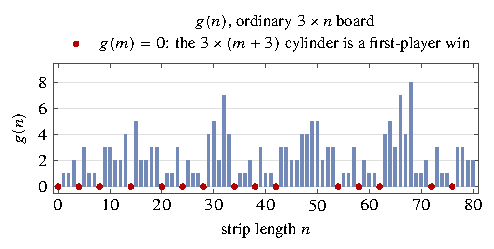
\includegraphics{figures/dawson_grundy.pdf}
\caption{Grundy values $g(n)$ of Dawson's chess on the $3\times n$ ordinary board (octal game
$\mathbf{0.137}$), $n\le80$. Dots mark $g(m)=0$: the $3\times m$ board is a second-player win and the
$3\times(m+3)$ cylinder a first-player win (Theorem~\ref{thm:ring}).}
\label{fig:dawson_grundy}
\end{figure}

The ring formula of~\cite{Study2025}, and its remark that the ring's value is 0 or 1, hold with the correct $g$
(Fig.~\ref{fig:dawson_grundy}). In mis\`ere play the ring rule carries over, since a forced sequence has odd
length (the first player wins exactly when the $(n-3)$-file strip is a mis\`ere P-position); our implementation of the Plambeck--Siegel algorithm~\cite{PlambeckSiegel2008} reproduces their partial
quotient for strips of at most 32 files (order 638, 109 P-positions) \lab{C2}, and the next quotient did not
finish (Section~S9).

\section{Engines and Sums}\label{sec:engines}

CGT suggests which endgames may trouble an engine: an infinitesimal such as ${\uparrow}$ is a fight over one
spare tempo and a nimber such as $\star$ a fight over parity; neither shows in the material, so a static
evaluation can miss them until the search sees the fight's end.

\subsection{A CGT Test Suite}

We built $233$ legal positions on the ordinary $8\times8$ board with at most seven men, each labeled by its CGT
class (Table~\ref{tab:sf}). In $181$ of them the Lichess tablebase~\cite{LichessTB} confirms the winning moves
that CGT predicts; in the other $52$ the model and the tablebase disagree, so we score the engines against the
tablebase.

\subsection{Stockfish and Lc0}

We ran Stockfish~19~\cite{Stockfish} on one thread with a $64$~MB hash and no tablebases. It solves all $233$
positions at $10^5$ nodes, and $232$ already at $10^3$ \lab{C1}. The classes separate at a small fixed depth
(Table~\ref{tab:sf}): at depth~1 the engine reads hot positions, numbers and switches correctly
$73$--$81\%$ of the time, but infinitesimals only $30\%$ ($26\%$ at depth~2) and nimbers $53\%$
\lab{C1}, consistent with tempo and parity fights, though nimbers and the class \emph{other} are not clearly
separated at this sample size. Both classes reach $100\%$ by depth~8.
With one engine and a small sample, this is a pilot.

\begin{table}[!t]
\centering
\caption{Stockfish~19 at Fixed Depth: Evaluations (\%) Matching the Tablebase, by CGT Class, Without the
Seven Decided ($\pm\BIG$) Positions}
\label{tab:sf}
\footnotesize
\begin{tabular}{@{}lrrrrrrr@{}}
\toprule
 & & \multicolumn{6}{c}{Search depth} \\
\cmidrule(l){3-8}
CGT class & $n$ & 1 & 2 & 4 & 6 & 8 & 12 \\
\midrule
hot ($\pm\BIG$ switch) & 68 & 81 & 78 & 91 & 97 & 99 & 100 \\
number & 57 & 79 & 81 & 84 & 93 & 95 & 98 \\
switch & 37 & 73 & 78 & 89 & 100 & 100 & 100 \\
other & 20 & 60 & 50 & 75 & 95 & 100 & 100 \\
nimber & 17 & 53 & 65 & 88 & 100 & 100 & 100 \\
infinitesimal & 27 & 30 & 26 & 59 & 85 & 100 & 100 \\
\bottomrule
\end{tabular}

\smallskip
\parbox{\columnwidth}{\footnotesize Infinitesimal: ups and downs, with or without $\star$. Other: values free of
$\BIG$ that fall in none of the other classes, such as tinies and games $\game{a\pm x}{b\pm y}$.}
\end{table}

Lc0~v0.32.1~\cite{Lc0}, with its bundled network, is perfect at all four budgets, $10^3$ to $10^6$ nodes,
all $17$ draws included \lab{C1}, so at practical budgets the suite is too easy for both engines.

\subsection{Engines on Sums}

Beyond seven men no tablebase applies, but CGT still values sums exactly. ChessSums is a set of $26{,}000$
pawn-endgame sums whose components come from a library of $418$ with $37$ distinct values, each the same in all
nine settings; whole-board alpha--beta confirms every outcome except five that hit its time limit \lab{C1}, an
independent minimax confirms $4{,}887$ \lab{C2}, and alpha--beta needs about $4$--$9$ times as many nodes per
added component \lab{C1}. We placed $200$ sums on the ordinary $8\times8$ board with a tr\'ebuchet on free
squares and ran both engines, but in $163$ of them the king group shares a file with the pawns, where the
frozen-king model need not hold, so we draw no conclusion from that test. On the $13$ positions where the group
stands clear of the pawns and a winning move exists, Stockfish~19 and Lc0 found one at every budget \lab{C1}. A
proper test of engines on sums is future work. A learning experiment on Dawson's chess is in Section~S9.

% \codeavail is defined in main.tex (named build: the repository URL; review build: anonymized).
% The fallback below only keeps this file compiling if main.tex does not define it.
\providecommand{\codeavail}{available at \expandafter\url\expandafter{\repourl}}

\section{Verification and Reproducibility}\label{sec:verify}

\emph{Cross-checks.} Our CGT engine agrees with a separate brute-force sum solver on $55{,}195$ positions $G$
(at most two pawns a side, $3$--$5$ files), for three race rules and $15$ reference games $R$: all
$4{,}967{,}550$ outcomes of $G+R$ match under the textbook test, e.p.\ on and off, and all $2{,}483{,}775$
under the e.p.-aware test. A whole-board minimax confirms its outcomes on $1{,}070$ single components. A Lean~4
project checks $123$ finite statements (Section~S17). AI models wrote the full \lab{S} proofs. AI referees, some from another vendor, checked them, and
programs ran the ring base cases; no human referee has yet.

\emph{Code and data availability.} The code and data are \codeavail. The supplementary material gives the
full proofs of the \lab{S} results (Sections~S12--S15) and the FEN of the main positions with kings (Section~S11).

\section{Conclusion and Open Problems}\label{sec:conclusion}

In the model, seven pawns on four files of the ordinary board make a $\nim{2}$ and no six do; nine make a
$\nim{3}$. On $2{,}049$ decisive $8\times8$ positions that we could solve (not a random sample) the model names the real winner in $92.5\%$; on six ranks a
square-rule passer test removes its pawn errors with frozen kings \lab{C1}. Section~S10 lists two more problems.

\begin{enumerate}
\item \emph{Higher nimbers.} Can a ring $\nim{3}$ on $\cyl{n}$ have only $n$ pawns (Fig.~\ref{fig:least})? Are
  the wall families $\nim{2}$ as sums for all $n$? Is there a $\nim{4}$ at any height?
\item \emph{Real chess.} With queen promotions and frozen kings the oracle value of the $1/8$ position is exactly
  $1/8$; does it survive all four promotions? The 8-man end positions deciding A and B agree with the model;
  those with 9 to 11 men are unsolved.
\item \emph{When is a tr\'ebuchet zero?} The certificate theory settles the promotion game, not chess. In the promotion
  game even a locked pawn pair can break a tr\'ebuchet's zero \lab{C2} (Section~S2).
\item \emph{Mis\`ere Dawson's chess.} Dawson asked about mis\`ere play \cite{Dawson1935}: is the mis\`ere
  quotient \cite{PlambeckSiegel2008} of Dawson's chess infinite? By the ring rule (Theorem~\ref{thm:ring}), an
  answer for strips also answers the cylinder.
\end{enumerate}


% The last page is short; keep its left column from being stretched to full height.
\raggedbottom
\section*{Acknowledgment}
\ifdefined\anonbuild
The authors thank
the maintainers of the Lichess tablebase, Stockfish and Lc0 for making their tools freely available. AI
coding assistants (Claude, Anthropic; Codex, OpenAI; and open models run through the OpenCode and Kilo tools)
wrote and ran, under the authors' direction, the software for the simulations, endgame searches, tablebases
and cross-checks of Sections~II--XIII and the scripts that draw the figures, and helped draft and edit the
text of all sections. The authors chose the research questions, directed the work and are responsible for all
content.
\else
The author thanks
Prof.~T.~Morley for mentoring the 2025 study on which this work builds, and
the maintainers of the Lichess tablebase, Stockfish and Lc0 for making their tools freely available. AI
coding assistants (Claude, Anthropic; Codex, OpenAI; and open models run through the OpenCode and Kilo tools)
wrote and ran, under the author's direction, the software for the simulations, endgame searches, tablebases
and cross-checks of Sections~II--XIII and the scripts that draw the figures, and helped draft and edit the
text of all sections. The author chose the research questions, directed the work and is responsible for all
content.
\fi


% (no \IEEEtriggeratref: both builds balance the last page without one)
\bibliographystyle{IEEEtran}
\bibliography{refs}

\end{document}
